\documentclass{lib/skripsi}

\usepackage{blindtext}
\usepackage{longtable}

%===========================================================
% Definisi Data Peneliti, Judul, Pembimbing dan Penguji
%-----------------------------------------------------------
\titleskripsi{IMPLEMENTASI FILTER SPASIAL LINEAR PADA VIDEO \textit{STREAM} MENGGUNAKAN \textit{FPGA HARDWARE ACCELERATOR}}

\fullname{SULAEMAN}
\idnum{H131 16 002}

\program{Sistem Informasi}
\dept{Matematika}
\faculty{Matematika dan Ilmu Pengetahuan Alam}
\university{Universitas Hasanuddin}
\city{Makassar}
\yearsubmit{2021}

\firstsupervisor{Dr. Eng. Armin Lawi, S.Si., M.Eng.}
\firstsupervisorNIP{197204231995121001}
\secondsupervisor{Supri Bin Hj Amir, S.Si., M.Eng.}
\secondsupervisorNIP{198805042019031012}
\firstexaminer{ Dr. Hendra, S.Si., M.Kom.}
\secondexaminer{ Nur Hilal A Syahrir, S.Si., M.Si.}

\degree{Sarjana Komputer}
\datesubmit{9}
\monthsubmit{April}
\headprogram{Dr. Muhammad Hasbi, M.Sc}
\headprogramNIP{196307201989031003}
%-----------------------------------------------------------
% End Definisi Data Peneliti, Judul, Pembimbing dan Penguji
%===========================================================

\begin{document}
    % HALAMAN SAMPUL
    \cover
    \pagenumbering{roman}
    
    % HALAMAN JUDUL
    \titlepage

    % PERNYATAAN KEOTENTIKAN
    \authenticationpage

    % LEMBAR PERSETUJUAN PEMBIMBING
    \supervisorapprovalpage

    % Halaman Pengesahan
    \approvalpage

    % KATA PENGANTAR
    \addcontentsline{toc}{chapter}{KATA PENGANTAR}
    \chapter*{KATA PENGANTAR}

Puji syukur penulis panjatkan kepada Allah SWT, karena atas berkat dan rahmat-Nya penulis dapat menyelesaikan skripsi ini. Shalawat serta salam senantiasa tercurah kepada \textit{Rasulullah} Muhammad \textit{Shallallahu Alaihi Wasallam,} yang merupakan teladan dalam menjalankan kehidupan dunia.

Alhamdulillah, skripsi dengan judul "IMPLEMENTASI FILTER SPASIAL LINEAR PADA VIDEO \textit{STREAM} MENGGUNAKAN \textit{FPGA HARDWARE ACCELERATOR}" yang disusun sebagai salah satu syarat untuk mencapai gelar Sarjana pada program studi Sistem Informasi fakultas Matematika dan Ilmu Pengetahuan Alam Universitas Hasanuddin ini dapat diselesaikan. Walaupun adanya kendala-kendala yang dihadapi khususnya wabah Covid-19 ketika skripsi ini dikerjakan. Tetapi dalam penulisan skripsi ini, penulis mampu menyelesaikan pada waktu yang tepat berkat bantuan dan dukungan dari berbagai pihak. 

Ucapan terima kasih dan apresiasi yang tak terhingga kepada kedua orang tua penulis bapak \textbf{Sudarmin} dan ibu \textbf{Yuli Hadiyanti} yang tak kenal lelah dalam memanjatkan doa serta memberikan nasihat dan motivasi kepada penulis. Tak lupa juga kepada saudara-saudara penulis \textbf{Fitri Handayani}, \textbf{Tri Novianti}, \textbf{Jumadil Yusuf}, \textbf{Muhammad Fitrah}, \textbf{Adam Ramadhan} yang selalu menjadi motivasi bagi penulis untuk terus melangkah maju.

Penulis menyadari bahwa skripsi ini dapat terselesaikan dengan adanya bantuan, bimbingan, dukungan dan motivasi dari berbagai pihak. Oleh karena itu, penulis mengucapkan ucapan terima kasih dengan tulus kepada:

\begin{enumerate}[topsep=0pt,itemsep=0pt,partopsep=0pt, parsep=0pt]
    \item Rektor Universitas Hasanuddin, Ibu \textbf{Prof. Dr. Dwia Aries Tina Pulubuhu} beserta jajarannya.
    \item Dekan Fakultas Matematika dan Ilmu Pengetahuan Alam, \textbf{Dr. Eng. Amiruddin} beserta jajarannya.
    \item Ketua Departemen Matematika FMIPA, \textbf{Dr. Nurdin, S.Si., M.Si}, dan juga \textbf{Dr. Muhammad Hasbi, M.Sc} sebagai ketua Program Studi Sistem Informasi Universitas Hasanuddin.
    \item Bapak \textbf{Dr. Eng. Armin Lawi, S.Si., M.Eng} sebagai pembimbing utama yang telah banyak memberikan arahan, ide, motivavsi serta dukungan kepada penulis dalam banyak hal.
    \item Almarhum bapak \textbf{Dr. Diaraya, M.Ak} dan bapak \textbf{Supri Bin Hj. Amir, S.Si., M.Eng} sebagi pembimbing pertama yang senantiasa  memberikan masukan kepada penulis.
    \item Bapak \textbf{Dr. Hendra, S.Si., M.Kom} dan Ibu \textbf{Nur Hilal, S.Si., M.Si} sebagai tim penguji atas saran dan masukan pada penelitian yang telah dilakukan oleh penulis.
    \item Seluruh Bapak dan Ibu dosen FMIPA Universitas Hasanuddin yang telah mendidik dan memberikan ilmunya sehingga penulis mampu menyelesaikan program sarjana. Serta para staf yang telah membantu dalam pengurusan berkas administrasi.

    \item Saudara-saudara \textbf{Ramsis Squad} \textbf{(Sultan, Muh Rizaldi, Sangereng Dewa Raja, Hajrin, Badaruddin Hidayat, Hamzah Julianto Nugraha, Muh Naim, Achmad Husein Nyompa)} sebagai keluarga semasa tinggal di Ramsis sejak menjadi mahasiswa baru, saling berbagi dalam banyak hal, saling membantu dan bahkan saling merepotkan.

    \item Saudara-saudara \textbf{Sunu Squad} dan \textbf{SSC Squad} \textbf{(Akbar, Muh Fikri Satria A, Andi Rezki Muh Nur, Muhammad Akbar Atori, Baharuddin Kasim, Andi Yaumil Falakh, Nur Ikhwan Putra Pratama, Bagas Prasetyo, Zinedine Kahlil Gibran Zidane, Rio Mukhtarom, Marfiandhi Putra, Abdul Aziz Mubarak,  Mutawally Syarawy, Fatur Rahman, Fitriadi Syawal Mustafa)} yang telah menemani penulis selama perkuliahan, saling memberi motivasi dan bantuan, meluangkan waktu dan berbagi suka-duka serta kebersamaan selama menuntut ilmu.

    \item Saudari \textbf{Suci Rahmadana Anwar} dan \textbf{Sri Juliana} yang senantiasa menemani, memberi nasihat, menjadi tempat bertanya, serta dukungan untuk menyelesaikan skripsi ini.

    \item Keluarga besar \textbf{Ilmu Komputer Unhas 2016} yang setia menemani dan membatu penulis selama menjalani pendidikan. Serta kakak-kakak dan adik-adik \textbf{Ilmu Komputer 2014, 2015, 2017, 2018} yang telah banyak membantu, semoga tetap semangat dalam mengejar impian.

    \item Keluarga besar \textbf{HIPERMAWA Koperti Unhas} yang senantiasa memberikan naungan kekeluargaan dan dukungan.

    \item Rekan-rekan \textbf{KKN Internasional Jepang Unhas Gel. 102} yang telah menjadi keluarga baru selama KKN dan menjadikan KKN sebagai momen yang berkesan.

    \item Serta semua pihak yang telah banyak berpartisipasi, baik secara langsung maupun tidak langsung dalam penyusunan skripsi ini yang tidak sempat penulis sebutkan satu per satu.
\end{enumerate}

Penulis menyadari bahwa skripsi ini masih jauh dari sempurna dikarenakan terbatasnya pengalaman dan pengetahuan yang dimiliki penulis. Oleh karena itu, penulis mengharapkan segala bentuk saran serta masukan bahkan kritik yang membangun dari berbagai pihak. Semoga tulisan ini memberikan manfaat kepada semua pihak yang membutuhkan dan terutama untuk penulis.

\vspace{1cm}
\begin{flushright}
    Makassar, 9 April 2021\\
    \vspace{2.5cm}
    {DENNY CHRISNANDA}\\
    NIM. {H13116002}
\end{flushright}


    \pagebreak

    % PERNYATAAN PERSETUJUAN PUBLIKASI
    \publicationapprovalpage

    % ABSTRAK
    \addcontentsline{toc}{chapter}{ABSTRAK}
    \chapter*{ABSTRAK}

Berbagai macam akselerator telah dikembangkan dalam meningkatkan kinerja dan efisiensi energi untuk menangani komputasi berat, salah satu diantaranya yaitu FPGA. FPGA mampu menangani beban komputasi yang begitu berat sehingga dapat digunakan untuk \textit{Digital Signal Processing}, \textit{Image Processing}, \textit{Neural Network}, dan sebagainya.
% metode
Pada penelitian ini penulis mencoba mengkaji kinerja yang dimiliki ARM prosesor dan FPGA pada FPGA \textit{Development Board} Xilinx PYNQ Z2 dalam penerapan filter spasial linear pada video \textit{stream}. Kernel filter yang digunakan pada penelitian ini yaitu \textit{average blur}, \textit{gaussian blur}, \textit{laplacian}, \textit{sharpen}, \textit{sobel horizontal} dan \textit{sobel vertical}. Parameter yang digunakan untuk mengukur kinerja ARM prosesor dan FPGA yaitu waktu komputasi, \textit{frame rate} (FPS), penggunaan CPU, penggunaan \textit{memory}, \textit{resident memory} (RES), \textit{shared memory} (SHR) dan \textit{virtual memory} (VIRT).
% hasil
Rata-rata waktu komputasi yang dibutuhkan untuk menerapkan filter spasial linear pada 200 frame dengan ARM prosesor adalah 29.06 detik sedangkan dengan FPGA rata-rata hanya dibutuhkan 3.32 detik. Waktu komputasi dengan FPGA 88.85\% lebih baik dibandingkan dengan ARM prosesor. Video hasil filter dengan ARM prosesor memperoleh rata-rata 6.95 fps sedangkan dengan FPGA rata-rata 60.37 fps. FPS dengan FPGA 88.49\% lebih baik lebih baik dibandingkan ARM prosesor. Penggunaan CPU pada FPGA 14.89\% lebih baik, penggunaan \textit{memory} pada FPGA 2.02\% lebih baik, penggunaan \textit{resident memory} 2.07\% lebih baik, dan penggunaan \textit{shared memory} 4.08\% lebih baik dibandingkan dengan ARM prosesor. Sedangkan penggunaan \textit{virtual memory} pada ARM prosesor 0.03\% lebih baik dibandingkan FPGA.


\begin{table}[h]
    \begin{tabular}{ p{0.17\textwidth} p{0.8\textwidth} }
        \\
        \textbf{Kata Kunci :} & filter spasial linear, FPGA, ARM prosesor, video \textit{stream}, \textit{video processing}
    \end{tabular}
\end{table}

 
    \pagebreak

    % ABSTRACT
    \addcontentsline{toc}{chapter}{ABSTRACT}
    \chapter*{ABSTRACT}

Various kinds of accelerators have been developed to improve performance and energy efficiency to handle heavy computations, one of which is FPGA. FPGA is capable of handling such a heavy computational load that it can be used for Digital Signal Processing, Image Processing, Neural Networks, etc. In this study, the authors tried to examine the performance of the ARM processor and the FPGA on the Xilin PYNQ Z2 FPGA Development Board in applying a linear spatial filter to the video stream. Kernel filters used in this study are the average blur, Gaussian blur, Laplacian, sharpen, Sobel horizontal, and Sobel vertical. The parameters used to measure the performance of ARM processors and FPGAs are runtime, frame rate (FPS), CPU usage, memory usage, resident memory (RES), shared memory (SHR), and virtual memory (VIRT). The average computation time required to apply linear spatial filters to 200 frames with an ARM processor is 29.06 seconds, while the average FPGA takes only 3.32 seconds. Compute time with FPGA is 88.85\% better than ARM processor. The filtered video with the ARM processor gets an average of 6.95 fps while the FPGA average is 60.37 fps. FPS with FPGA is 88.49\% better than ARM processor. CPU usage on FPGA is 14.89\% better, memory usage on FPGA is 2.02\% better, usage of resident memory is 2.07\% better, and usage of shared memory is 4.08\% better than ARM processor. While the use of virtual memory on ARM processors is 0.03\% better than FPGA. 


\begin{table}[h]
    \begin{tabular}{ p{0.17\textwidth} p{0.8\textwidth} }
        \\
        \textbf{Keywords :} & linear spatial filter, FPGA, ARM processor, video stream, video processing
    \end{tabular}
\end{table}
    \pagebreak

    %===========================================================
    % Daftar isi, daftar gambar, daftar tabel
    %-----------------------------------------------------------
    \addcontentsline{toc}{chapter}{DAFTAR ISI}
    \tableofcontents
    \pagebreak

    \addcontentsline{toc}{chapter}{DAFTAR TABEL}
    \listoftables
    \pagebreak

    \addcontentsline{toc}{chapter}{DAFTAR GAMBAR}
    \listoffigures
    \pagebreak

    \addcontentsline{toc}{chapter}{DAFTAR LAMPIRAN}
    \listofappendices
    \pagebreak

    \pagenumbering{arabic}
    %-----------------------------------------------------------
    % End Daftar isi, daftar gambar, daftar tabel
    %===========================================================

    %===========================================================
    % Daftar masukan untuk Bab
    %-----------------------------------------------------------
    \chapter{Pendahuluan}

\section{Latar Belakang Masalah}
FUXA merupakan salah satu perangkat lunak SCADA (Supervisory Control and Data Acquisition) sumber terbuka yang banyak digunakan dalam berbagai aplikasi industri. Namun, hingga saat ini FUXA belum secara resmi mendukung protokol \textit{Factory Interface Network Service} (FINS) yang dikembangkan oleh Omron.

Di sisi lain, industri manufaktur yang mengandalkan \textit{Programmable Logic Controller} (PLC) dari Omron memerlukan sistem visualisasi data secara \textit{real-time} yang kompatibel dengan protokol komunikasi FINS. Ketiadaan dukungan ini menyebabkan keterbatasan integrasi antara sistem SCADA open-source dan perangkat keras dari Omron.

Oleh karena itu, diperlukan upaya pengembangan modul komunikasi FINS pada FUXA agar sistem SCADA ini mampu berkomunikasi secara efektif dengan PLC Omron, sehingga dapat digunakan secara luas oleh industri dan komunitas pengembang perangkat lunak terbuka.

\section{Rumusan Masalah}
Rumusan masalah dalam penelitian ini adalah sebagai berikut:
\begin{enumerate}
    \item Bagaimana menambahkan dukungan protokol FINS pada FUXA dengan fitur yang setara dengan protokol lain seperti Modbus?
    \item Bagaimana memastikan proses pembacaan dan penulisan data melalui protokol FINS berjalan stabil serta dapat ditampilkan dengan benar pada antarmuka pengguna (UI)?
\end{enumerate}

\section{Tujuan dan Manfaat Penelitian}
\subsection{Tujuan Penelitian}
Penelitian ini bertujuan untuk mengimplementasikan dukungan protokol FINS pada FUXA, meliputi:
\begin{itemize}
    \item Pengambilan data secara berkala (polling),
    \item Penulisan nilai ke PLC,
    \item Dukungan \textit{Data Acquisition} (DAQ),
    \item Integrasi sistem alarm berbasis tag.
\end{itemize}

\subsection{Manfaat Penelitian}
Manfaat dari penelitian ini antara lain:
\begin{itemize}
    \item Menyediakan solusi SCADA sumber terbuka yang kompatibel dengan PLC Omron, khususnya untuk industri kecil dan menengah.
    \item Memberikan kontribusi nyata dalam pengembangan perangkat lunak sumber terbuka di bidang otomasi industri.
\end{itemize}

\section{Ruang Lingkup Penelitian}
Penelitian ini memiliki ruang lingkup sebagai berikut:
\begin{itemize}
    \item Fokus pada implementasi komunikasi FINS melalui protokol UDP/TCP.
    \item Penggunaan area memori standar PLC Omron seperti \texttt{DM}, \texttt{CIO}, \texttt{W}, dan sejenisnya.
    \item Pengembangan terbatas pada pembacaan dan penulisan tag serta visualisasi nilai melalui UI FUXA.
    \item Pengujian dilakukan menggunakan perangkat lunak analisis jaringan seperti Wireshark serta PLC fisik maupun simulator.
\end{itemize}

\section{Hipotesis Penelitian}
Hipotesis dari penelitian ini adalah:
\begin{itemize}
    \item Jika protokol FINS berhasil diintegrasikan ke dalam FUXA, maka sistem SCADA tersebut akan mampu membaca dan menulis data dari PLC Omron secara stabil dan akurat.
    \item Performa polling dan DAQ yang dihasilkan akan setara dengan protokol komunikasi lain seperti Modbus.
\end{itemize}

\section{Sistematika Penulisan}
Adapun sistematika penulisan dalam laporan ini adalah sebagai berikut:
\begin{itemize}
    \item \textbf{Bab 1} – Pendahuluan: berisi latar belakang, rumusan masalah, tujuan dan manfaat, ruang lingkup, hipotesis, dan sistematika penulisan.
    \item \textbf{Bab 2} – Tinjauan Referensi: membahas teori dan referensi terkait, seperti protokol FINS, FUXA, dan komunikasi industri.
    \item \textbf{Bab 3} – Metodologi Penelitian: menjelaskan tahapan dan metode penelitian yang digunakan.
    \item \textbf{Bab 4} – Implementasi dan Pengujian: menyajikan proses integrasi FINS pada FUXA serta hasil pengujian.
    \item \textbf{Bab 5} – Kesimpulan dan Saran: berisi simpulan dari hasil penelitian serta rekomendasi untuk pengembangan lebih lanjut.
\end{itemize}

    \chapter{TINJAUAN PUSTAKA}

\section{Landasan Teori}

\subsection{Perusahaan Manufaktur dan Kebutuhan Otomasi}
Industri manufaktur modern sangat bergantung pada sistem otomasi untuk meningkatkan efisiensi produksi, konsistensi kualitas, dan pengendalian biaya. Otomasi industri melibatkan penggunaan perangkat keras seperti sensor, aktuator, dan Programmable Logic Controller (PLC) yang terhubung ke sistem kontrol dan pengawasan seperti SCADA (Supervisory Control and Data Acquisition) \parencite{sastoque2023assessing}.

Perusahaan seperti \textit{Special Purpose Machine (SPM) Maker} sering kali merancang dan membangun mesin otomatis untuk kebutuhan spesifik di pabrik. Mesin-mesin ini biasanya menggunakan PLC dari berbagai vendor, termasuk Omron, Siemens, dan Allen-Bradley. Untuk memantau dan mengendalikan mesin secara efisien, diperlukan sistem HMI dan SCADA yang andal, fleksibel, dan mudah diintegrasikan dengan protokol komunikasi industri \parencite{humaj2021fins}.

\subsection{Programmable Logic Controller (PLC)}
PLC adalah perangkat digital berbasis mikroprosesor yang dirancang untuk mengontrol proses otomatis di lingkungan industri. PLC dapat diprogram untuk menjalankan logika kontrol yang kompleks dan sangat tahan terhadap kondisi ekstrem seperti getaran, suhu tinggi, dan interferensi listrik. PLC berfungsi sebagai otak dari sistem otomasi, mengumpulkan data dari sensor dan mengontrol aktuator berdasarkan logika yang telah diprogram \parencite{emqx2023fins}.

\subsection{Protokol Komunikasi Industri dan FINS}
Agar PLC dapat terhubung ke perangkat lain, diperlukan protokol komunikasi industri. Protokol ini memungkinkan transfer data secara real-time antara PLC dan SCADA. Contoh protokol yang umum digunakan antara lain Modbus, OPC UA, Profibus, EtherNet/IP, dan FINS \parencite{sastoque2023assessing}.

FINS (Factory Interface Network Service) merupakan protokol yang dikembangkan oleh Omron untuk memungkinkan komunikasi antar perangkat di dalam jaringan otomasi industri \parencite{humaj2021fins}. FINS mendukung komunikasi melalui UDP dan TCP. Kelebihan FINS antara lain:
\begin{itemize}
    \item Kompatibel dengan semua seri PLC Omron.
    \item Dukungan komunikasi jarak jauh melalui pengalamatan jaringan.
    \item Struktur data fleksibel, seperti area CIO, DM, WR, HR.
\end{itemize}

\subsection{SCADA dan DAQ dalam Konteks Industri}
SCADA adalah sistem yang digunakan untuk mengontrol dan memonitor proses industri secara terpusat. SCADA mencakup fungsi utama seperti akuisisi data (DAQ), kontrol jarak jauh, alarm, logging historis, dan visualisasi data melalui HMI \parencite{uddin2022open}. Akuisisi data (DAQ) berperan penting dalam mengumpulkan nilai-nilai sensor dan status proses secara periodik, yang kemudian disimpan dan dianalisis untuk pengambilan keputusan.

Polling adalah metode yang digunakan oleh SCADA untuk mengambil data dari perangkat lapangan seperti PLC. Dalam polling, sistem SCADA mengirim permintaan ke PLC secara berkala dan membaca respon data yang dikirimkan kembali \parencite{omidi2023node}.

\subsection{HMI dan Visualisasi Data}
HMI (Human-Machine Interface) adalah antarmuka antara manusia dan sistem kontrol. HMI menyediakan representasi visual dari proses industri dan memungkinkan operator untuk memantau kondisi sistem dan melakukan intervensi jika diperlukan. Fitur penting dalam HMI meliputi grafik waktu nyata, pengaturan parameter, tampilan alarm, dan trend historis \parencite{seeed2024fuxa}.

\subsection{Teknologi Web Modern: HTML, CSS, JavaScript, TypeScript, Node.js, Angular}
Perkembangan teknologi web memungkinkan sistem HMI dan SCADA dikembangkan sebagai aplikasi web lintas platform yang dapat diakses melalui browser secara real-time. Teknologi utama yang digunakan antara lain:

\begin{itemize}
    \item \textbf{HTML (HyperText Markup Language)}: Bahasa standar untuk menyusun struktur dan elemen-elemen dasar halaman web.
    
    \item \textbf{CSS (Cascading Style Sheets)}: Digunakan untuk mendesain tampilan visual halaman web, termasuk warna, tata letak, dan responsivitas antarmuka.
    
    \item \textbf{JavaScript}: Bahasa pemrograman inti untuk interaktivitas pada web, memungkinkan manipulasi DOM, penanganan event, dan komunikasi asynchronous melalui AJAX.
    
    \item \textbf{TypeScript}: Merupakan superset dari JavaScript yang dikembangkan oleh Microsoft, menyediakan fitur pengetikan statis dan pemrograman berorientasi objek yang kuat. TypeScript digunakan secara luas dalam pengembangan Angular karena meningkatkan skalabilitas, keamanan, dan maintainability kode.
    
    \item \textbf{Node.js}: Platform berbasis JavaScript yang berjalan di sisi server (backend). Node.js mendukung arsitektur non-blocking dan event-driven, sehingga sangat cocok untuk aplikasi SCADA yang membutuhkan performa tinggi dan komunikasi data real-time.
    
    \item \textbf{Angular}: Framework frontend modern yang dikembangkan oleh Google. Angular menggunakan TypeScript sebagai bahasa utamanya dan menyediakan pendekatan pengembangan berbasis komponen, dependency injection, serta routing yang efisien. Angular mempermudah pembuatan antarmuka pengguna (HMI) yang dinamis, modular, dan responsif.
    
    \item \textcite{emmanni2025typescript} menjelaskan bagaimana penggunaan TypeScript dalam pengembangan framework JavaScript modern seperti Angular meningkatkan keandalan dan skalabilitas aplikasi SCADA berbasis web.
    
    \item \textcite{scarsbrook2023typescript} menyoroti keunggulan TypeScript dalam meningkatkan keamanan tipe dan produktivitas tim pengembang dalam proyek perangkat lunak berskala besar, termasuk sistem SCADA.

\end{itemize}

Dengan kombinasi teknologi tersebut, sistem SCADA berbasis web menjadi lebih fleksibel, ringan, dan dapat diakses lintas perangkat tanpa memerlukan instalasi perangkat lunak tambahan \parencite{seeed2024fuxa}.

\subsection{SCADA Open-Source dan Vendor Lock-In}
Salah satu tantangan utama dalam dunia industri adalah ketergantungan terhadap vendor atau \textit{vendor lock-in}. Sistem SCADA komersial umumnya bersifat tertutup dan berlisensi mahal, sehingga membatasi fleksibilitas pengguna dalam hal integrasi, migrasi, maupun penyesuaian sistem.

Vendor lock-in menyebabkan pengguna hanya dapat menggunakan layanan, protokol, atau perangkat lunak dari penyedia tertentu, sehingga sulit untuk beralih ke penyedia lain tanpa mengeluarkan biaya besar atau menghadapi gangguan layanan. Dalam konteks cloud computing, fenomena ini bahkan menjadi lebih kritis, karena banyak organisasi bergantung pada layanan seperti DBaaS (Database-as-a-Service). Ketika organisasi membutuhkan fitur baru atau terjadi perubahan harga, ketergantungan ini menjadi hambatan besar untuk berpindah platform \parencite{banthia2024vendorlockin}.

Untuk mengatasi vendor lock-in, banyak organisasi mulai mengadopsi pendekatan berbasis teknologi terbuka dan strategi multi-cloud. Salah satu solusi yang relevan dalam konteks SCADA adalah penggunaan sistem open-source seperti FUXA. Dengan menggunakan SCADA open-source, pengguna memperoleh kendali penuh atas kode sumber, arsitektur, dan kemampuan integrasi sistem, sehingga meminimalkan risiko dikunci oleh vendor tertentu.

FUXA adalah contoh SCADA berbasis web yang bersifat open-source dan mendukung berbagai protokol industri seperti Modbus, OPC-UA, dan MQTT. Sistem ini dapat dikustomisasi secara penuh dan tidak tergantung pada penyedia perangkat lunak tertentu \parencite{seeed2024fuxa}.

\subsection{Electron: Aplikasi Desktop Berbasis Web}
Electron adalah framework open-source yang memungkinkan pengembangan aplikasi desktop lintas platform (Windows, macOS, dan Linux) menggunakan teknologi web seperti HTML, CSS, dan JavaScript, dikombinasikan dengan Node.js dan Chromium. Framework ini banyak digunakan untuk membangun aplikasi desktop modern karena kemampuannya menjalankan kode frontend dan backend dalam satu kerangka kerja yang terintegrasi \parencite{electron2024why}.

Beberapa keunggulan utama Electron antara lain:

\begin{itemize}
\item \textbf{Lintas platform}: Aplikasi yang dikembangkan dengan Electron dapat berjalan di berbagai sistem operasi tanpa perlu penulisan kode ulang.
\item \textbf{Teknologi web modern}: Memanfaatkan ekosistem luas dari JavaScript, TypeScript, dan pustaka web.
\item \textbf{Stabil dan enterprise-grade}: Digunakan oleh perusahaan besar seperti Microsoft (Visual Studio Code), OpenAI (ChatGPT Desktop), Discord, dan Slack.
\item \textbf{Kemudahan integrasi native}: Mendukung pemanggilan kode native (C++, Rust, dsb) jika diperlukan.
\end{itemize}

Dengan bundling Chromium dan Node.js, Electron memberikan kendali penuh terhadap tampilan dan fungsionalitas aplikasi desktop, sekaligus menghindari keterbatasan atau bug dari webview bawaan sistem operasi \parencite{electron2024why}.

\subsection{Pengujian dan Validasi Sistem SCADA}
Pengujian (testing) merupakan bagian penting dalam pengembangan sistem SCADA. Pengujian bertujuan untuk memastikan sistem dapat membaca dan menulis data secara benar, menangani kondisi ekstrem, serta menampilkan visualisasi data yang akurat. Pengujian biasanya mencakup:

\begin{itemize}
    \item \textbf{Unit testing}: Memastikan setiap komponen bekerja sesuai fungsi.
    \item \textbf{Integration testing}: Memastikan komunikasi antara komponen berjalan lancar.
    \item \textbf{System testing}: Menguji sistem secara menyeluruh dalam kondisi nyata atau simulasi.
    \item \textbf{Network traffic analysis}: Menggunakan Wireshark atau alat sejenis untuk memantau paket FINS dalam jaringan \parencite{almas2014open}.
\end{itemize}

\section{Penelitian Terdahulu}

\subsection{Implementasi SCADA Open-Source dalam Industri}
Beberapa studi telah membuktikan efektivitas SCADA open-source dalam dunia industri:


\begin{itemize}
\item \textcite{uddin2022open} mengembangkan SCADA berbasis Node-RED dan Grafana untuk sistem reverse osmosis tenaga surya.
\item \textcite{omidi2023node} menggunakan SCADA open-source untuk pembangkit listrik hibrid, menekankan efisiensi energi.
\item \textcite{almas2014open} menunjukkan integrasi SCADA open-source dengan PMU dan protokol DNP3.
\item \textcite{rubiomedrano2023icsnet} menerapkan FUXA pada honeynet ICSNet untuk mensimulasikan serangan siber industri.
\item \textcite{abbas2015efficient} mengusulkan protokol komunikasi SCADA yang efisien untuk otomasi industri guna mengurangi latensi dan meningkatkan integritas data.
\item \textcite{eras_almeida2023off_grid_pv} melakukan evaluasi kinerja SCADA open-source dalam sistem pembangkit tenaga surya off-grid, dengan fokus pada keandalan monitoring dan kontrol sistem energi terdistribusi.
\end{itemize}
\subsection{Implementasi SCADA pada Sistem Otomatisasi Rumah}
Sistem SCADA tidak hanya digunakan pada industri manufaktur skala besar, tetapi juga mulai diimplementasikan dalam sistem otomasi rumah (smart home). Penelitian oleh Hazdi et al. (2017) menunjukkan bagaimana SCADA berbasis web dapat dirancang untuk memantau dan mengendalikan sistem rumah secara otomatis menggunakan PLC dan antarmuka berbasis browser \parencite{hazdi2017scada}. Sistem ini menunjukkan fleksibilitas SCADA dalam skala kecil serta potensi adaptasinya untuk kebutuhan rumah tangga atau industri kecil.

\subsection{Pemanfaatan FUXA dalam Pendidikan dan Simulasi}
FUXA juga digunakan secara luas dalam pendidikan dan penelitian, antara lain:

\begin{itemize}
    \item Visualisasi data sensor menggunakan MQTT dan Raspberry Pi \parencite{seeed2024fuxa}.
    \item Penggunaan dalam laboratorium simulasi sistem kontrol.
    \item Integrasi dengan PLC simulasi dan HMI desain interaktif.
\end{itemize}

    \chapter{METODOLOGI PENELITIAN}

\section{Jenis Penelitian}
Jenis penelitian ini adalah penelitian rekayasa perangkat lunak (software engineering research), yang bertujuan untuk merancang, mengimplementasikan, dan mengevaluasi penambahan dukungan protokol FINS (Factory Interface Network Service) pada sistem SCADA open-source FUXA. Penelitian ini bersifat terapan dengan pendekatan kuantitatif dan kualitatif dalam menguji fungsionalitas dan performa sistem.

\section{Metode Pengembangan Sistem}
Metode yang digunakan dalam pengembangan perangkat lunak ini adalah metode iteratif dan inkremental, dengan tahapan sebagai berikut:

\begin{enumerate}
    \item \textbf{Analisis Kebutuhan:} Mengidentifikasi kebutuhan pengguna terhadap integrasi protokol FINS pada FUXA, termasuk dukungan konfigurasi parameter (DA1, SA1, Unit Address), polling tag, penulisan nilai ke PLC, serta fitur DAQ dan alarm.
    \item \textbf{Perancangan Sistem:} Mendesain struktur konektor FINS di sisi server dan antarmuka pengguna di sisi client, sesuai dengan arsitektur FUXA (Node.js dan Angular).
    \item \textbf{Implementasi:} Mengembangkan modul konektor FINS (server/runtime/devices/fins), komponen konfigurasi tag dan perangkat (Angular), serta logika polling dan penulisan data.
    \item \textbf{Pengujian dan Evaluasi:} Melakukan pengujian fungsional, integrasi, serta monitoring paket FINS menggunakan Wireshark untuk memastikan komunikasi berjalan benar.
    \item \textbf{Perbaikan dan Optimalisasi:} Menangani error, optimasi performa polling, memory leak (EventEmitter), serta penambahan fitur lanjutan (alarm, DAQ).
\end{enumerate}

\section{Alat dan Bahan}
\begin{itemize}
    \item \textbf{Perangkat Keras:} Laptop/PC, jaringan LAN, PLC Omron (atau simulator).
    \item \textbf{Perangkat Lunak:}
          \begin{itemize}
              \item FUXA (https://github.com/frangoteam/FUXA)
              \item Node.js, Angular CLI, Git
              \item Wireshark untuk sniffing paket FINS
              \item Visual Studio Code untuk pengembangan
          \end{itemize}
    \item \textbf{Library Tambahan:}
          \begin{itemize}
              \item \texttt{node-omron-fins} atau modifikasi client FINS custom
              \item Angular Material untuk UI komponen konfigurasi
          \end{itemize}
\end{itemize}

\section{Tahapan Penelitian}
Penelitian dilakukan dalam beberapa tahap berikut:

\begin{table}[H]
    \centering
    \begin{tabular}{|c|p{8cm}|}
        \hline
        \textbf{No} & \textbf{Kegiatan}                                                 \\
        \hline
        1           & Studi literatur tentang protokol FINS, SCADA, dan arsitektur FUXA \\
        2           & Perancangan konektor dan struktur konfigurasi perangkat/tag       \\
        3           & Implementasi modul konektor dan antarmuka pengguna                \\
        4           & Pengujian komunikasi, pengamatan melalui Wireshark                \\
        5           & Evaluasi dan dokumentasi hasil integrasi                          \\
        \hline
    \end{tabular}
    \caption{Tahapan Pelaksanaan Penelitian}
\end{table}

\section{Platform dan Arsitektur Aplikasi}
Dalam pengembangan aplikasi SCADA berbasis web untuk desktop, penulis menggunakan framework \textbf{Electron} sebagai pembungkus (wrapper) yang mengemas aplikasi Angular dan Node.js ke dalam executable lintas platform. Dengan pendekatan ini, sistem dapat dijalankan sebagai aplikasi desktop independen tanpa perlu instalasi web server terpisah maupun browser.

Arsitektur ini memberikan keuntungan berupa:
\begin{itemize}
    \item Kemudahan distribusi dan instalasi.
    \item Akses langsung terhadap sistem file dan perangkat lokal.
    \item Performa tinggi karena menggunakan versi terbaru Chromium dan V8 engine.
    \item Kemandirian penuh dari browser atau runtime eksternal.
\end{itemize}

Penggunaan Electron menjadikan aplikasi SCADA dapat digunakan di lingkungan industri yang membutuhkan portabilitas, kestabilan, serta kontrol penuh terhadap platform distribusi.

\subsection{Topologi Sistem dan Komunikasi FINS}

Topologi sistem yang direncanakan dalam penelitian ini digambarkan pada Gambar \ref{fig:topologi}. Diagram tersebut memvisualisasikan arsitektur konektivitas yang akan dikembangkan antara perangkat lunak SCADA sumber terbuka (FUXA) yang dijalankan pada Mini PC dengan delapan PLC Omron CJ2M yang merepresentasikan delapan pos kerja pada suatu lini produksi. Setiap PLC akan dihubungkan melalui jaringan lokal menggunakan protokol FINS berbasis UDP/TCP. Selain itu, sistem dirancang untuk menampilkan informasi performa produksi secara waktu nyata melalui LCD TV yang terhubung langsung ke Mini PC sebagai media dashboard utama.

\begin{figure}[H]
    \centering
    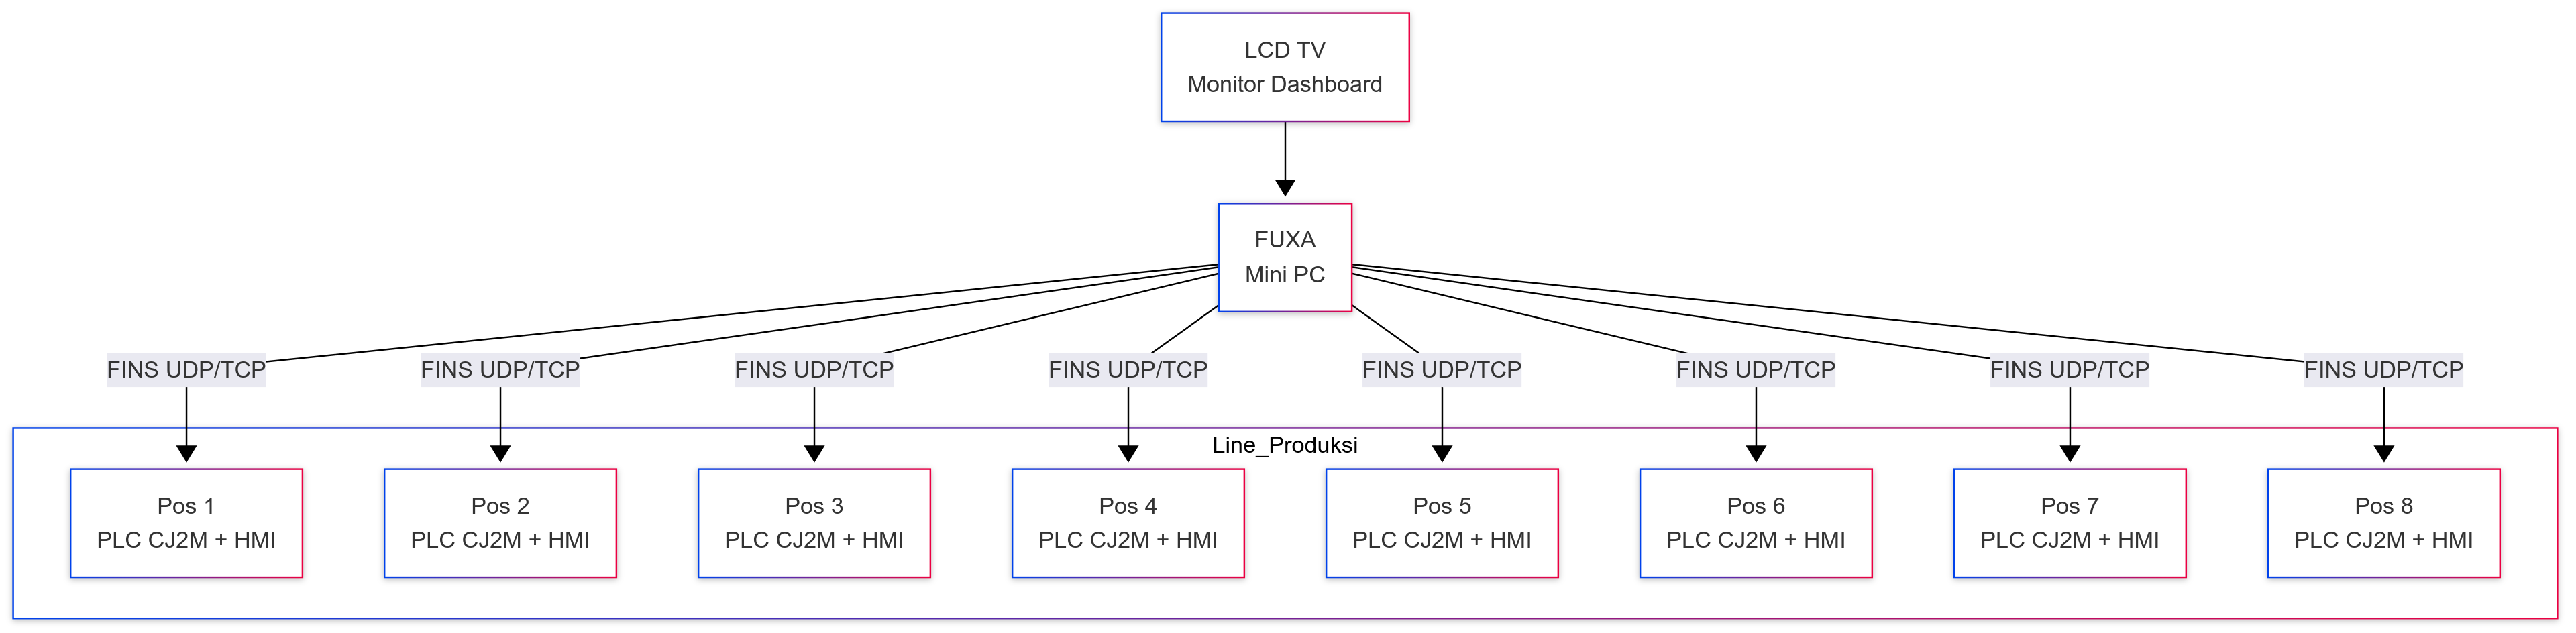
\includegraphics[width=\textwidth]{images/topologi_fuxa_fins.png} % Ganti dengan nama file SVG/PNG diagram hasil ekspor dari Mermaid
    \caption{Topologi Sistem SCADA FUXA dengan Protokol FINS}
    \label{fig:topologi}
\end{figure}

Diagram ini juga menunjukkan bahwa Mini PC berperan sebagai pusat kendali yang mengatur komunikasi ke setiap titik kontrol (posisi 1 sampai 8) di jalur produksi. Setiap posisi memiliki kombinasi PLC CJ2M dan HMI yang menangani proses otomatisasi lokal. Informasi yang dikumpulkan dan dianalisis oleh FUXA dapat disajikan secara waktu nyata melalui tampilan TV dashboard untuk kebutuhan pemantauan operator.

\section{Metode Pengujian}

Pengujian dilakukan untuk memastikan bahwa integrasi protokol FINS pada sistem SCADA FUXA berjalan dengan benar dan andal. Metode pengujian dibagi menjadi dua pendekatan utama, yaitu \textit{black-box testing} dan \textit{white-box testing}, sebagaimana dijelaskan berikut ini:

\subsection{Black-Box Testing}

Pengujian \textit{black-box} berfokus pada aspek fungsional sistem dari sudut pandang pengguna tanpa melihat struktur internal kode. Tujuan utama pengujian ini adalah untuk memverifikasi apakah sistem bekerja sesuai dengan yang diharapkan.

\begin{itemize}
    \item \textbf{Pengujian Konfigurasi Perangkat:} Memastikan bahwa parameter seperti \texttt{DA1}, \texttt{SA1}, \texttt{Unit Address}, dan \texttt{protocol} dapat disimpan dan ditampilkan ulang dengan benar.
    \item \textbf{Pengujian Pembacaan Data:} Mengamati apakah nilai dari PLC dapat ditampilkan di UI (user interface) FUXA secara waktu nyata setelah polling.
    \item \textbf{Pengujian Penulisan Data:} Menguji kemampuan sistem dalam mengubah nilai tag pada PLC dari UI, dan memastikan nilai benar-benar tersimpan di memori PLC.
    \item \textbf{Pengujian Alarm:} Mengaktifkan kondisi pemicu alarm dan mengevaluasi apakah notifikasi muncul sesuai logika yang ditetapkan.
    \item \textbf{Pengujian DAQ:} Memverifikasi apakah data historis disimpan dengan benar dalam sistem logging dan dapat ditampilkan kembali.
    \item \textbf{Pengujian Antarmuka:} Memastikan setiap komponen UI dapat diakses dan tidak menimbulkan error saat digunakan.
\end{itemize}

\subsection{White-Box Testing}

Pengujian \textit{white-box} dilakukan dengan menganalisis struktur internal dari sistem, termasuk logika program, alur data, serta penggunaan sumber daya. Pengujian ini membantu dalam menemukan error tersembunyi dan masalah performa.

\begin{itemize}
    \item \textbf{Unit Testing Konektor FINS:} Menguji fungsi-fungsi internal pada modul \texttt{server/runtime/devices/fins} seperti \texttt{connect()}, \texttt{read()}, \texttt{write()}, dan \texttt{poll()}.
    \item \textbf{Pengujian Event Emitter:} Mengevaluasi apakah listener pada konektor dibersihkan dengan benar untuk menghindari \textit{memory leak} akibat listener ganda.
    \item \textbf{Pengujian Error Handling:} Mengaktifkan simulasi gangguan komunikasi dan melihat apakah mekanisme retry atau error recovery berjalan dengan baik.
    \item \textbf{Logging dan Debug Output:} Memastikan bahwa log debug dapat memberikan informasi cukup untuk pelacakan kesalahan (tracing).
    \item \textbf{Pengamatan Trafik Jaringan:} Menggunakan Wireshark untuk memverifikasi bahwa paket FINS dikirim dan diterima sesuai dengan struktur protokol, termasuk header, command code, dan respons yang sesuai.
    \item \textbf{Integrasi Client-Server:} Menyusuri alur data dari UI (Angular) ke Node.js backend untuk menjamin komunikasi antar komponen berlangsung tanpa error.
\end{itemize}
    \chapter{HASIL DAN PEMBAHASAN}
    
\chapter{KESIMPULAN DAN SARAN}


\section{Kesimpulan}
% \subsection{Citra Digital}
\blindtext

\section{Saran}
\blindtext
    %-----------------------------------------------------------
    % End Daftar masukan untuk Bab
    %===========================================================

    %===========================================================
    % Daftar Pustaka
    %-----------------------------------------------------------
    \addcontentsline{toc}{chapter}{DAFTAR PUSTAKA}
    \printbibliography[title={DAFTAR PUSTAKA}]
    %-----------------------------------------------------------
    % End Daftar Pustaka
    %===========================================================
    
    %===========================================================
    % Daftar Lampiran
    %-----------------------------------------------------------
    \appendix
    \addcontentsline{toc}{chapter}{LAMPIRAN}
    \addtocontents{toc}{\protect\setcounter{tocdepth}{0}}
    \chapter*{LAMPIRAN}

    %-----------------------------------------------------------
    % End Daftar Lampiran
    %===========================================================

\end{document}